\documentclass{beamer}
\usepackage{listings}
\usepackage{graphicx}
\graphicspath{ {./images/} }
\lstset{
%language=C,
frame=single, 
breaklines=true,
columns=fullflexible
}
\usepackage{subcaption}
\usepackage{url}
\usepackage{tikz}
\usepackage{tkz-euclide} % loads  TikZ and tkz-base
%\usetkzobj{all}
\usetikzlibrary{calc,math}
\usepackage{float}
\newcommand\norm[1]{\left\lVert#1\right\rVert}
\providecommand{\brak}[1]{\ensuremath{\left(#1\right)}}
\providecommand{\abs}[1]{\vert#1\vert}
\providecommand{\fourier}{\overset{\mathcal{F}}{ \rightleftharpoons}}
\providecommand{\pr}[1]{\ensuremath{\Pr\left(#1\right)}}
\providecommand{\sbrak}[1]{\ensuremath{{}\left[#1\right]}}
\renewcommand{\vec}[1]{\mathbf{#1}}
\usepackage[export]{adjustbox}
\usepackage[utf8]{inputenc}
\usepackage{amsmath}
\usepackage{mhchem}
\usetheme{Boadilla}

\title{PROBABILITY FUSION FOR HYPERSPECTRAL AND LIDAR DATA}
\subtitle{by \\ Chiru Ge, Sthandong Normal University, China \\Qian Du, Mississippi State University, USA}
\author{Presented by: S.Goutham Sai}
\institute{IITH(CSE)}
\date{\today}
\begin{document}

\begin{frame}
    \titlepage
\end{frame}

\begin{frame}{Abstract}
    In this paper, a new probability fusion strategy is proposed for hyperspectral and LiDAR data classification, which is inspired by the representation residual fusion strategy in our previous works. Unlike the residual fusion strategy which utilizes a collaborative representation classifier, the probability fusion strategy deploys a deep residual network(DRN). This paper compares the two fusion strategies. The experiment results show that the probability fusion strategy with the DRN is better than the residual fusion strategy in classification performance.
\end{frame}

\begin{frame}{Keyterms}
      \begin{block}{Hyperspectral Image}
        A hyperspectral image is an image which contains the continuous sprectrum of every pixel in the image. It is done with the purpose of finding objects, identifying materials, or detecting processes.
    \end{block}
      \begin{block}{LiDAR}
        LiDAR stands for "laser imaging, detection, and ranging".It is a method for determining ranges (variable distance) by targeting an object with a laser and measuring the time for the reflected light to return to the receiver.     
      \end{block}
      \begin{block}{Residual Fusion}
        Residual fusion is another fusion strategy proposed by the authors in their previous works. It uses the framework of collaborative representation based classification. 
    \end{block}
\end{frame}

\begin{frame}{Keyterms}
    \begin{block}{Local Binary Pattern}
        Local binary patterns (LBP) is a type of visual descriptor used for classification in computer vision. LBP is the particular case of the Texture Spectrum model proposed in 1990
    \end{block}
\end{frame}

\begin{frame}{Introduction}
\begin{itemize}
    \item Multi-source remote sensing images contain detailed information about the ground. For e.g., LiDAR which contains information about the height and shape information, Hyperspectral Images (HSI) with spectral information. 
    \item HSI and LiDAR images contain complementary information. Hence fusing the two data sources can further improve classification performance.
    \item However, automatic data fusion is still challenging. This fusion can be achieved by feature level fusion or decision level fusion.
    \item Many works of the feature level fusion involve the step of dimensionality reduction , which can lead to a feature selection problem.
    \item To utilize the entire datasets or all features, residual fusion is proposed, which belongs to the decision level fusion.
\end{itemize}
\end{frame}

\begin{frame}{Introduction}
    \begin{itemize}
        \item Inspired by the residual fusion strategy, a novel probability fusion method with the deep residual network(DRN) is proposed which can has the advantage of residual fusion and can achieve higher classification accuracy.
    \item The main contributions of this paper are:
    \begin{enumerate}
        \item The paper proposes a new method based on probability fusion for the fusion of HSI and LiDAR image.
        \item The probability fusion framework can be extended to any spatial features and any deep learning network structures for HSI and LiDAR data fusion.
        \item The performance of residual fusion and probability fusion is fairly compared with the previous work on collaborative representation.
    \end{enumerate}
    \end{itemize}
\end{frame}

\begin{frame}{Methodology}
    \begin{itemize}
        \item In the residual fusion framework, spatial features are first extracted. Spatial features are the stacked features of the Extinction profile(EP) and local binary pattern(LBP) due to their effectiveness.
        \item Then, the HSI spectral features, HSI spatial features and LiDAR spatial features aew normalized because different sources of data generally have different value ranges.
        \item Next, each source of data  is input into a collaborative representation-based classifier with Tikhonov regularization(KCRT) classifier to obtain the residuals.
        \begin{block}{Tikhonov regularization}
            Tikhonov regularization, named for Andrey Tikhonov, is a method of regularization of ill-posed problems. 
        \end{block}
        \item Finally the residuals are fused to acquire the reconstruction residual that can be used finalize the class membership of a testing pixel. 
    \end{itemize}
\end{frame}

\begin{frame}{Methodology}
    \begin{itemize}
        \item Let $r(y) = [r_1(y),r_2(y), \dots ,r_l(y), \dots r_C(y)]$ be the residual vector for a testing sample y, where C is the total number of classes.
        \item The equation of residual fusion can be written as:
        \begin{align}
            r(y) = abr_{HSI}(y) + b(1-a)r_{HSI\_EPLBP}(y) + (1-b)r_{LiDAR\_EPLBP}(y)
        \end{align}
        where a and b $\rightarrow$ weighting parameters, $r_{HSI}(y),r_{HSI\_EPLBP}(y),r_{LiDAR\_EPLBP}(y) \rightarrow$ residual vectors from HSI Spectral features, HSI spatial features and LiDAR spatial features respectively.
        \item The class label of y can be calculated using:
        \begin{align}
            class(y) = arg\ min_{l = 1, \dots C}\big(r(y)\big)
        \end{align}
    \end{itemize}
\end{frame}

\begin{frame}{Methodology}
    \begin{itemize}
        \item Let $p(y) = [p_1(y),p_2(y), \dots ,p_l(y), \dots p_C(y)]$ be the probability vector for a testing sample y.
        \item The equation of residual fusion can be written as:
        \begin{align}
            r(y) = cdp_{HSI}(y) + d(1-c)p_{HSI\_EPLBP}(y) + (1-d)p_{LiDAR\_EPLBP}(y)
        \end{align}
         where c and d $\rightarrow$ weighting parameters, $p_{HSI}(y),p_{HSI\_EPLBP}(y),p_{LiDAR\_EPLBP}(y) \rightarrow$ probability vectors from HSI Spectral features,HSI spatial features and LiDAR spatial features respectively.
        \item The class label of y can be calculated using:
        \begin{align}
            class(y) = arg\ max_{l = 1, \dots C}\big(p(y)\big)
        \end{align}
        \item The advantage of probability fusion and residual fusion is that they both can correct the wrong labels of single-source data. However, both the methods have two sensitive parameters to be tuned.
    \end{itemize}
\end{frame}

\begin{frame}{Methodology}
    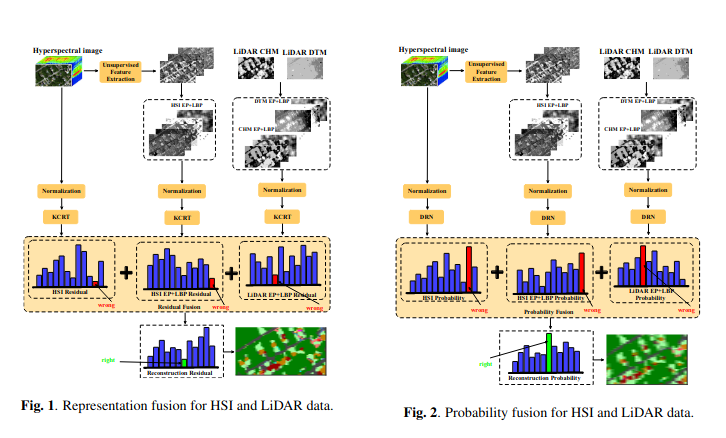
\includegraphics[scale=0.5]{fig_1_and_2}
\end{frame}

\begin{frame}{Methodology}
    \begin{enumerate}
        \item Fig. 1 shows a testing sample of the seventh class, which was  misclassified  by  three  classifiers  utilizing  every  single source, but accurately classified by the representation residual fusion method.
        \item Fig.   2  depicts  our  proposed  probability  fusion  for  HSI and  LiDAR  images,  which  was  inspired  by  representation residual fusion.  The difference is that probability fusion utilizes  DRN  to  classify  each  source  of  data,  and  the  testing pixel is assigned to the class with the largest fused probability. DRN acquires the probability matrices of each source. Finally, three probability matrices are fused to obtain the reconstruction probability that can be utilized to finalize the class label of a testing sample.
    \end{enumerate}
\end{frame}

\begin{frame}{Experiments}
    \begin{block}{Experiment Data}
        \begin{itemize}
            \item Wertheim data come from Goddard’s LiDAR, Hyperspectral,and Thermal (G-LiHT) data.  The G-LiHT Airborne Imager[6]  supplies  co-registered  LiDAR  DTM,  LiDAR  CHM,  LiDAR Point Cloud, hyperspectral reflectance image at 1m spatial resolution and google earth overlay by Keyhole Markup Language (KML) at 0.25m spatial resolution.
            \item Experiments are conducted on the HSI,CHM and DTM data which were collected in June 2016 across the Wertheim region(geographical coordinate is at $40^o 46' 30''$latitude,$−72^o 52' 48''$longitude)).
            \item The  hyperspectral  image  has  114 bands with a spectral range of 420 nm to 950 nm. Spatial resolution of HSI, CHM, and DTM is 1 m. The data set of the entire scene contains $501\times 1523$ pixels.  
            \item There are 5 categories are in the Wertheim data. Table 1 shows these categories and the corresponding number of training, validation, and testing samples.
        \end{itemize}
    \end{block}
\end{frame}

\begin{frame}{Experiments}
    \begin{table}[h!]
        \centering
        \scalebox{0.8}{
        \resizebox{\textwidth}{!}{
        \begin{tabular}{|c|c|c|c|c|}
            \hline 
            \hline
            & Class & \multicolumn{3}{|c|}{Number of Samples}\\
            \hline
            No & Name & Training & Validation & Testing \\
            \hline
            1 & Tree & 811 & 969 & 177163 \\
            2 & Sea & 182 & 224 & 10416 \\
            3 & Sand & 130 & 135 & 4548 \\
            4 & Commercial &96 & 95 & 1024 \\
            5 & Pool/Water & 50 & 44 & 191 \\
            6 & Major thoroughfares & 334 & 382 & 4604 \\
            7 & Bare soil & 326 & 328 & 6230 \\
            8 & Road & 372 & 370 & 6893 \\
            9 & Parking lot & 191 & 163 & 1458 \\
            10 & Grass & 296 & 303 & 2890 \\
            11 & Residential grey & 116 & 119 & 725 \\
            12 & Residential coffee & 144 & 144 & 1271 \\
            13 & Solar panel & 30 & 30 & 95 \\
            14 & Car & 116 & 113 & 420 \\
            15 & Electric wire & 138 & 140 & 1052 \\
            \hline
            & Total & 3332 & 3559 & 218980
        \end{tabular}
        }}
        \caption{Wertheim: number of training, validation and testing samples}
        \label{tab:1}
    \end{table}
\end{frame}

\begin{frame}{Experiments}
    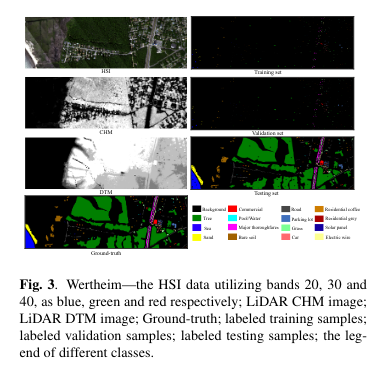
\includegraphics[scale=0.4]{fig3}
    \begin{block}{Parameter setting}
        \begin{itemize}
            \item Appropriate parameters of KCRT and DRN need to be set.But, due to the limited space, the detailed parameter tuning process of KCRT and DRN is not shown.
         \end{itemize}
    \end{block}
\end{frame}

\begin{frame}{Experiments}
    \begin{block}{Parameter setting}
     \begin{itemize}
         \item Fig.   4 shows  the parameter tuning  process for  residual fusion and probability fusion. 
         \begin{center}
            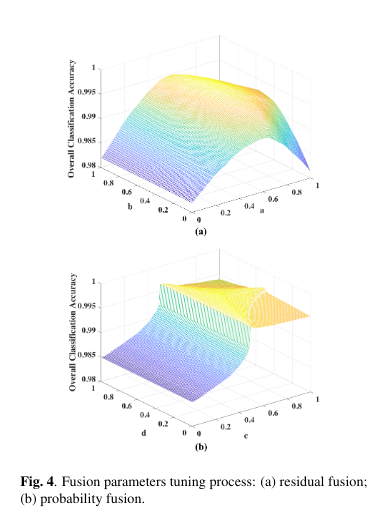
\includegraphics[scale =0.4]{fig4}
         \end{center}
     \end{itemize}
    \end{block}
\end{frame}

\begin{frame}{Experiments}
    \begin{block}{Parameter Setting}
      \begin{itemize}
          \item For residual fusion parameters a and b,  the optimal parameter are selected through Fig.   4(a):a = 0.71 and b = 0.66.
          \item For probability fusion, the best parameters c = 0.48 and d = 0.62.
          \item In  the  experiments,  common  classification  metrics,  i.e.,AA, OA, Kappa are utilized.
      \end{itemize}
    \end{block}
    \begin{block}{Results}
    \begin{itemize}
        \item Table  2  shows  classification  results  of  residual  fusion.   As we can see, residual fusion offers higher classification accuracy than using each individual source, which illustrates the validity of residual fusion.
        \item Table 3 shows classification results of our proposed probability fusion.  As we can see, classification accuracy of probability fusion is higher than that of each source, which illustrates the validity of probability fusion.
    \end{itemize}
    \end{block}
\end{frame}

\begin{frame}{Experiments}
    \begin{block}{Results}
    \begin{center}
        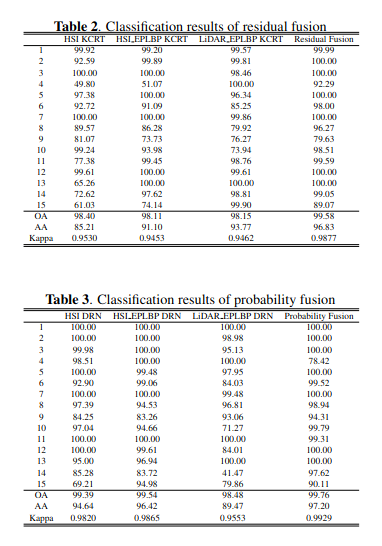
\includegraphics[scale=0.4]{tables}
    \end{center}
    \end{block}
\end{frame}

\begin{frame}{Experiments}
    \begin{block}{Results}
        \begin{itemize}
            \item Compared with Table 2, classification accuracy of probability fusion is higher than that of residual fusion.  The reason is that the classification performance of DRN is superior to KCRT.
            \begin{center}
                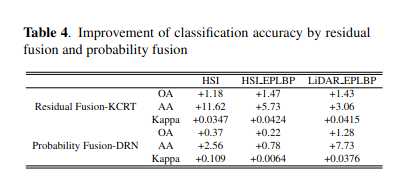
\includegraphics[scale=0.4]{table4}
            \end{center}
            \item Table 4 shows improved classification accuracy by residual fusion and probability fusion,  compared with the corresponding counterpart using all the sources.
            \item Table 4 presents that  residual  fusion  improves  classification  accuracy  more than probability fusion, which demonstrates the potential of residual fusion.
        \end{itemize}
    \end{block}
\end{frame}

\begin{frame}{Experiments}
    \begin{block}{Results}
        \begin{itemize}
            \item To summarize, residual fusion and probability fusion are both useful for HSI and LiDAR data fusion classification. Although  probability  fusion  with  DRN is  better  than  residualfusion with KCRT in performance, residual fusion combined with  a  better  representation classifier  may  further  improve performance.
        \end{itemize}
    \end{block}
\end{frame}

\begin{frame}{Conclusion}
    A  new  probability  fusion  strategy  is  proposed  for  HSI  and LiDAR data fusion.  Our proposed probability fusion framework  can  be  extended  to  any  spatial  features  and  any  deep learning network structures for HSI and LiDAR data fusion.The experimental results show that the DRN-based probability fusion outperforms the KCRT-based representation residual fusion.
\end{frame}

\end{document}